\paragraph{Complexiteit}
De complexiteit van de library valt goed mee, dankzij de beschikbare documentatie van de library is het zeer 
gemakkelijk om alle mogelijkheden van de library terug te vinden en zelf in een project te implementeren. 

\paragraph{Herbruikbaarheid}
\begin{figure}[H]
    \centering
    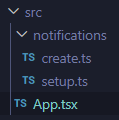
\includegraphics[height=0.1\textheight]{notificationsschaalbaarheidcross.png}
    \caption{Structuur notificaties implementatie React Native.}
\end{figure}
Door de logica van de library op te delen is het gemakkelijk om later opnieuw dezelfde logica op andere plaatsen 
in de code te gebruiken. Er moet enkel een methode geïmporteerd worden om een notificatie aan te maken. Aan die methode 
wordt dan de titel en beschrijving meegegeven. Het is ook mogelijk om de logica voor het aanmaken van een notificatie 
aan te passen. Dit kan dan gemakkelijk gebeuren in het \textbf{create.ts} bestand. Of er kan een nieuwe methode worden 
aangemaakt om bijvoorbeeld de notificatie in te plannen op een later tijdstip.